
\documentclass[DIV=calc, paper=a4, fontsize=11pt, twocolumn, spanish]{scrartcl}	 % A4 paper and 11pt font size

\usepackage{lipsum} % Used for inserting dummy 'Lorem ipsum' text into the template
\usepackage[protrusion=true,expansion=true]{microtype} % Better typography
\usepackage{amsmath,amsfonts,amsthm} % Math packages
\usepackage[svgnames]{xcolor} % Enabling colors by their 'svgnames'
\usepackage[hang, small,labelfont=bf,up,textfont=it,up]{caption} % Custom captions under/above floats in tables or figures
\usepackage{booktabs} % Horizontal rules in tables
\usepackage{fix-cm}	 % Custom font sizes - used for the initial letter in the document
\usepackage[spanish]{babel}
\selectlanguage{spanish}
\usepackage{hyperref}
\usepackage[utf8]{inputenc}
\usepackage{graphicx}

\usepackage{sectsty} % Enables custom section titles
\allsectionsfont{\usefont{OT1}{phv}{b}{n}} % Change the font of all section commands

\usepackage{fancyhdr} % Needed to define custom headers/footers
\pagestyle{fancy} % Enables the custom headers/footers
\usepackage{lastpage} % Used to determine the number of pages in the document (for "Page X of Total")

% Headers - all currently empty
\lhead{}
\chead{}
\rhead{}

% Footers
\lfoot{}
\cfoot{}
\rfoot{\footnotesize Page \thepage\ of \pageref{LastPage}} % "Page 1 of 2"

\renewcommand{\headrulewidth}{0.0pt} % No header rule
\renewcommand{\footrulewidth}{0.4pt} % Thin footer rule

\usepackage{lettrine} % Package to accentuate the first letter of the text
\newcommand{\initial}[1]{ % Defines the command and style for the first letter
\lettrine[lines=3,lhang=0.3,nindent=0em]{
\color{DarkGoldenrod}
{\textsf{#1}}}{}}

%----------------------------------------------------------------------------------------
%	TITLE SECTION
%----------------------------------------------------------------------------------------

\usepackage{titling} % Allows custom title configuration

\newcommand{\HorRule}{\color{DarkGoldenrod} \rule{\linewidth}{1pt}} % Defines the gold horizontal rule around the title

\pretitle{\vspace{-30pt} \begin{flushleft} \HorRule \fontsize{35}{35} \usefont{OT1}{phv}{b}{n} \color{DarkRed} \selectfont} % Horizontal rule before the title

\title{Campo eléctrico I: líneas de campo} % Your article title

\posttitle{\par\end{flushleft}\vskip 0.2em} % Whitespace under the title

\preauthor{\begin{flushleft}\large \lineskip 0.5em \usefont{OT1}{phv}{b}{sl} \color{DarkRed}} % Author font configuration

\author{Sebastián Valencia, } % Your name

\postauthor{\footnotesize \usefont{OT1}{phv}{m}{sl} \color{Black} % Configuration for the institution name
Universidad de los Andes \\ 201111578

\par\end{flushleft}\HorRule} % Horizontal rule after the title



\date{} % Add a date here if you would like one to appear underneath the title block

%----------------------------------------------------------------------------------------

\begin{document}

\maketitle % Print the title

\thispagestyle{fancy} % Enabling the custom headers/footers for the first page 

%----------------------------------------------------------------------------------------
%	ABSTRACT
%----------------------------------------------------------------------------------------

% The first character should be within \initial{}
\initial{E}\textbf{n este experimento observamos con la ayuda de un voltimetro las lineas de campo que se establecen entre pares de objetos cargados. Las sondas del voltimetro están montadas sobre un compás cuya orientación coincide con la dirección de la linea de campo correspondiente cuando la diferencia de potencial registrada máxima (en valor absoluto).}\\

\textbf{Para las lineas de campo encontradas verificamos si son iguales las sumas de las diferencias de potencial a lo largo de ellas, siendo esto una consecuencia del carácter conservativo de los campos eléctricos, y del comportamiento de campos electrostáticos de objetos conductores.}

%----------------------------------------------------------------------------------------
%	ARTICLE CONTENTS
%----------------------------------------------------------------------------------------

\section*{Objetivos}

\begin{itemize}
\item Encontrar y analizar las lineas de campo eléctrico que se establecen entre pares de objetos conductores cargados.

\item Verificar aspectos del carácter conservativo de los campos eléctricos.
\end{itemize}


\section*{Marco teórico}

La definición de campo eléctrico, es directamente análoga, y posee la misma motivación a la de un campo gravitatorio, estudiado en los primeros cursos de mecánica Newtoniana. Un campo eléctrico $E$, en cualquier punto o ubicación del espacio, es hallado posicionando una partícula de prueba con carga $q$ en ese punto. El vector de campo $\hat{E} = \hat{F} / q$, donde $\hat{F}$ es la fuerza eléctrica sobre la partícula de prueba. 

\begin{figure}[htbp]
\centering
	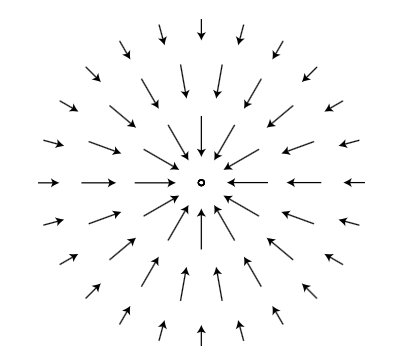
\includegraphics[scale=0.8]{data/img/field}
	\caption{Un ejemplo de carga negativa, aquí, la partícula con carga $q^-$, es un sumidero de lineas de campo eléctrico.}
\end{figure}

Las cargas, son la fuerza motora o generadora de los campos eléctricos. A diferencia de la gravedad, la cual es atractiva, la electricidad despliega atracción y repulsión. Una carga positiva $q^+$ es un fuente de campos eléctricos, mientras una carga negativa $q^-$, es un sumidero.


\section*{Procedimiento experimental}

Ubicamos un par de objetos en la cubeta, cada uno de ellos conectado a uno de los bornes de la fuente de voltaje. Al objeto conectado a la terminal negativa lo llamamos cátodo, y al conectado a la positiva lo llamamos ánodo. La cubeta tiene una delgada capa de agua, posiblemente con algo de sal, que actúa como agente conductor.\\

Fijamos en el compás las sondas del voltimetro de tal forma que la separación entre ellas sea de mas o menos 4 cm. Ademas nos aseguramos de que el voltimetro este configurado en DC.\\

\begin{figure}[htbp]
\centering
	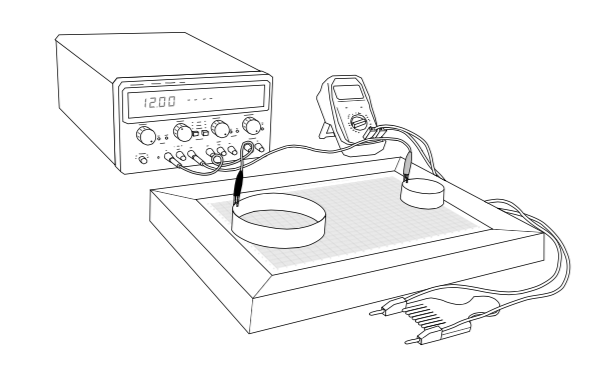
\includegraphics[scale=0.8]{data/img/experiment}
	\caption{Disposición experimental}
\end{figure}

Sumergimos las sondas del voltimetro en la cubeta comenzando con la sonda COM tan cerca como sea posible al cátodo. La sonda COM se mantiene fija, y la otra se gira hasta que se obtiene la máxima diferencia de potencial; en este instante la orientación del compás coincide aproximadamente con la orientación de la linea de campo en esa región. Registramos en una reproducción a escala 1:1 las posiciones de las sondas y la diferencia de potencial. Luego desplazamos la sonda COM al lugar donde en el paso anterior termino la sonda giratoria, y repetimos el procedimiento hasta llegar tan cerca como sea posible al ánodo.\\

Para terminar de registrar todas las diferencias de potencial cuando vamos del cátodo al ánodo, liberamos del compás a las sondas del voltimetro, medimos la diferencia de potencial entre la superficie del cátodo y la posición donde se ubicó por primera vez la sonda COM; también medimos la diferencia de potencial entre la superficie del ánodo y la posición donde quedó por ultima vez la sonda giratoria.

\section*{Cuestionario}

\begin{itemize}
\item ¿Cuales son las características de los campos eléctricos en la superficie de objetos conductores?

En general, los materiales son neutros, es decir sus átomos contienen tantas cargas positivas en el núcleo, como electrones en la corteza, sin embargo, en los metales los electrones pueden tener movilidad dentro de la red cristalina.\\

 En lo que respecta al comportamiento eléctrico, los materiales pueden dividirse en dos categorías: conductores y aislantes o dieléctricos. Un conductor metálico es un solido que contiene electrones libres, llamados electrones de conducción, que pueden desplazarse en el interior de la materia, pero no pueden dejar la superficie.\\
 
 
El campo eléctrico dentro de un conductor en equilibrio (dentro del metal) debe ser nulo o de lo contrario el campo forzaría el movimiento de los electrones de conducción; la única solución electrostática posible es que el campo sea cero en todo punto del interior del conductor. \\

$$|\hat{E}| = 0$$

El interior de un conductor en equilibrio, debe ser una región a voltaje constante. Es decir, $V$ no puede variar de un punto a otro al tener $|\hat{E}| = 0$. (\url{http://www.heurema.com/ApuntesFQ/AFisica/CampoElectrico/Campo\%20el\%E9ctrico\%20en\%20conductores.pdf})

$$|V| = cte$$

\item Consulte el manual de la fuente de voltaje, lea la sección “Getting Started” y la sub-sección “Constant Voltage / Constant Current Crossover”; haga un resumen.

El generador o fuente, posee tres modos de operación: 

\begin{enumerate}
\item Independiente, las fuentes de corriente y voltaje, son controladas y entregadas de manera independiente.
\item En serie, las fuentes son entregadas en serie, permitiendo la entrega de más corriente, voltaje o energía.
\item Paralelas, ambas fuentes de cada tipo, se conectan en paralelo.
\end{enumerate}

En la disposición \textit{Constant Voltage / Constant Current Crossover}, se permite transmisión constante de ambas magnitudes físicas mientras la carga cambia, hasta obtener la no constante en el límite permitido por el fabricante.
\end{itemize}

%----------------------------------------------------------------------------------------

\end{document}